\documentclass[9pt,toc=listof,paper=portrait,paper=24cm:17cm,mpinclude=true,captions=outerbeside,usegeometry=true,\jobname]{scrbook}
\usepackage{geometry} %[showframe]

\areaset{10cm}{18.8cm}
\setlength{\columnsep}{\marginparsep}   % the columnsep is used by KOMA captionbeside to separate the caption from the image

\savegeometry{defaultpage}

%\usepackage[english]{babel}
\usepackage[utf8]{inputenc}

\usepackage{polyglossia}
\usepackage{csquotes}
\setmainlanguage{english}

\usepackage[table]{xcolor}
\usepackage{ragged2e}                           % RaggedLeft and RaggedRight commands (left align, right align)
\usepackage[hang]{footmisc}                     % hanging footnote, possible ragged but this introduces new breaks and consequently new pages
\usepackage{url}
\usepackage{hyperref}                           % references in PDF
\usepackage{fnpct}                              % footnotes and punctuation make 1. -> .1
\usepackage{graphicx}                           % Include images
\usepackage{caption}
\usepackage{subcaption}                         % for subfigure
\usepackage{newfloat}                           % for \DeclareFloatingEnvironment
\usepackage[section]{placeins}                  % https://tex.stackexchange.com/questions/279/how-do-i-ensure-that-figures-appear-in-the-section-theyre-associated-with
\usepackage[natbib=true,backend=biber,style=alphabetic-verb]{biblatex}
\usepackage{mparhack}                           % For the right placement of marginpars. https://www.texfaq.org/FAQ-marginparside
\usepackage{xparse}                             % for environments
\usepackage[strict]{changepage}                 % for wider then the typearea
\usepackage{shorttoc}
\usepackage{calc}                               % for geometry calculations



\usepackage{listings}
\usepackage{booktabs,subcaption,amsfonts,dcolumn}
\newcolumntype{d}[1]{D..{#1}}
\newcommand\mc[1]{\multicolumn{1}{c}{#1}}
%\usepackage{booktabs}
\setlength{\heavyrulewidth}{1.5pt}
\setlength{\abovetopsep}{4pt}
\usepackage{ amssymb }
%%%%%%%%%%%%%%%
\usepackage{comment}
%\pgfplotsset{width=10cm,compat=1.9}
\usepackage{graphicx}
\usepackage{xcolor}
\usepackage{pgf-pie}
\usepackage{amsmath}
\usepackage{booktabs}
\usepackage{cleveref}                           % provides \cref command
\usepackage{todonotes}
\usepackage{lststyles}
\usepackage{paralist}
\usepackage{tikz}
\usetikzlibrary{shapes,arrows,positioning,fit,backgrounds}
\newcommand{\hsp}{\vphantom{Ag}}
\usepackage{xspace}
\usepackage{multirow}

\usepackage{import} % For /subimport{./}{sibling-file.tex}

\setuptodonotes{inline}


% <lsq2-commands>
\newcommand{\dbpedia}{\textsc{DBpedia}\xspace}
\newcommand{\linkedgeodata}{\textsc{LinkedGeoData}\xspace}
\newcommand{\swdf}{\textsc{SWDF}\xspace}
\newcommand{\wikidata}{\textsc{Wikidata}\xspace}

\newcommand{\biotrdf}{\textsc{Bio2RDF}\xspace}
\newcommand{\affymetrix}{\textsc{Affymetrix}\xspace}
\newcommand{\biomodels}{\textsc{BioModels}\xspace} % aka biomedels
\newcommand{\ctd}{\textsc{CTD}\xspace}
\newcommand{\dbsnp}{\textsc{dbSNP}\xspace}
\newcommand{\drugbank}{\textsc{DrugBank}\xspace}
\newcommand{\genage}{\textsc{GenAge}\xspace}
\newcommand{\gendr}{\textsc{GenDR}\xspace}
\newcommand{\go}{\textsc{GO}\xspace} % aka gene
\newcommand{\goa}{\textsc{GOA}\xspace}
\newcommand{\hgnc}{\textsc{HGNC}\xspace}
\newcommand{\irefindex}{\textsc{iRefIndex}\xspace}
\newcommand{\kegg}{\textsc{KEGG}\xspace}
\newcommand{\linkedspl}{\textsc{LinkedSQP}\xspace}
\newcommand{\mgi}{\textsc{MGI}\xspace}
\newcommand{\ncbigene}{\textsc{NCBIGene}\xspace}
\newcommand{\omim}{\textsc{OMIM}\xspace}
\newcommand{\pharmgkb}{\textsc{PharmGKB}\xspace}
\newcommand{\sabiork}{\textsc{SABIORK}\xspace}
\newcommand{\sgd}{\textsc{SGD}\xspace}
\newcommand{\sider}{\textsc{SIDER}\xspace}
\newcommand{\taxonomy}{\textsc{Taxonomy}\xspace}
\newcommand{\wormbase}{\textsc{Wormbase}\xspace}
% </lsq2-commands>

% <sparklify>
\usepackage[ruled,vlined, linesnumbered]{algorithm2e}
\usepackage{tabularx}
\usepackage{booktabs}
\usepackage{fancybox}
\usepackage{colortbl}

\newcommand{\fixme}[2][Fixme]{\textcolor{red}{\textbf{[#1:}} {\color{blue} {#2}}\textcolor{red}{\textbf{]}}}
\newcommand{\furl}[1]{\footnote{\scriptsize \url{#1}}}

\newcounter{metric}
\newcommand{\emphb}[1]{\textbf{\textit{#1}}}
\newcommand{\defn}[1]{\emphb{#1}\quad}
\newcommand\newitem[1][]{\item[#1)]\refstepcounter{metric}\def\@currentlabel{#1}}

\definecolor{cycle3}{RGB}{77, 175, 74}
\newcommand{\win}{\cellcolor{cycle3!30}}

% </sparklify>


% <maven-based-data-mgmt>
\usepackage{microtype}
\usepackage[newfloat]{minted}

%\newcommand{\textls}[1]{#1}% Note additional group!
\renewcommand{\textls}[1]{#1}
% "normal" (i.e. non-raised) tilde (~) symbols in minted enviroment
\setminted[]{fontfamily=lmtt}

% </maven-based-data-mgmt>


% <linkedgeodata>
%\usepackage[T1]{fontenc}
\usepackage{array}
\usepackage{threeparttable}
\usepackage{tabulary} %can use align in tables with line breaks
\usepackage{sepnum}
\usepackage{longtable}
\usepackage{algpseudocode}
%\usepackage{underscore}
%\usepackage[english]{babel} % use german Umlaute in examples

%\DeclareCaptionType{algorithmic}

\newcommand{\val}[1]{\sepnum{.}{\,}{}{#1}}
\newcommand{\valunit}[2]{\val{#1}\,#2}
\newcommand{\valrange}[2]{\val{#1} -- \val{#2}}
\newcommand{\valunitrange}[3]{\val{#1} -- \valunit{#2}{#3}}

%\newcommand{\todo}[1]{\textbf{[ToDo: #1]}}
\newcommand{\torev}[1]{\textbf{[Review: #1]}}

\renewcommand{\algorithmicrequire}{\textbf{Input:}}
\renewcommand{\algorithmicensure}{\textbf{Output:}}

%\newcommand{\algorithmicrequire}{\textbf{Input:}}
%\newcommand{\algorithmicensure}{\textbf{Output:}}

% </linkedgeodata>


% <simplified-r2rml>
\lstdefinestyle{rdf}{numberblanklines=true, morekeywords={}}
\lstdefinestyle{sparql}{numberblanklines=true, morekeywords={SELECT, WHERE, FILTER, GROUP, BY, IN, AS, SERVICE, GRAPH}}
\newcommand{\urlfn}[1]{\footnote{\scriptsize\url{#1}}}
% <simplified-r2rml>

\setlength{\footnotemargin}{\parindent}

% draw frame around the complete page
%\usepackage{eso-pic}
%\AddToShipoutPictureBG{\begin{tikzpicture}[overlay,remember picture]
% \draw (current page.south west) rectangle (current page.north east);
%\end{tikzpicture}}

%% Configure Bibliography
\addbibresource{references.bib}
\DeclareRefcontext{web}{labelprefix=Web:}

\setsansfont{Open Sans}[
UprightFont = {* Condensed Light},
ItalicFont = {* Condensed Light Italic},
BoldFont = {* Condensed Bold},
]

\setkomafont{pageheadfoot}{\large\sffamily}
\setkomafont{pagenumber}{\large\sffamily}

% For more caption customization
% https://tex.stackexchange.com/a/318175/11820

\captionsetup[listing]{name={Listing}}

\captionsetup{format=plain, labelfont={bf}, font=footnotesize}
% , singlelinecheck=off

% \begin{disfigure}[short title]{long title}{label}
%   content
% \end{disfigure}
% Stared for wide figures
\NewDocumentEnvironment{disenv}{ o m m }
{
  \checkoddpage
  \ifoddpage
    %odd
    \captionsetup{justification=RaggedRight}
  \else
    %even
    \captionsetup{justification=RaggedLeft}
  \fi
  \begin{captionbeside}%
  [\IfValueTF{#1}{#1}{#2}]% short title
  {#2\label{#3}}
  [o]% caption on the outer document side
  [\dimexpr\textwidth+\marginparwidth+\marginparsep\relax]% enlarge the used width
  [0pt]*% align with the inner margin
  \begin{minipage}[b]{\textwidth}
}
{
  \end{minipage}
  \end{captionbeside}
}
\NewDocumentEnvironment{disenv*}{ o m m }
{
  \begin{adjustwidth*}{}{\dimexpr-\marginparwidth+\marginparsep\relax}
%  \begin{minipage}[b]{\dimexpr\textwidth+\marginparwidth+\marginparsep\relax}
}
{
  \end{adjustwidth*}
  \caption[\IfValueTF{#1}{#1}{#2}]{#2}
  \label{#3}
}

\NewDocumentEnvironment{disfigure}{ o m m }
{
  \begin{figure}[htbp]
    \begin{disenv}[#1]{#2}{#3}
}
{
    \end{disenv}
  \end{figure}
}
\NewDocumentEnvironment{disfigure*}{ o m m }
{
  \begin{figure}[htbp]
    \begin{disenv*}[#1]{#2}{#3}
}
{
    \end{disenv*}
  \end{figure}
}

\NewDocumentEnvironment{dislisting}{ o m m }
{
  \begin{listing}[htbp]
    \begin{disenv}[#1]{#2}{#3}
}
{
    \end{disenv}
  \end{listing}
}
\NewDocumentEnvironment{dislisting*}{ o m m }
{
  \begin{listing}[htbp]
    \begin{disenv*}[#1]{#2}{#3}
}
{
    \end{disenv*}
  \end{listing}
}

\NewDocumentEnvironment{distable}{ o m m }
{
  \begin{table}[htbp]
    \begin{disenv}[#1]{#2}{#3}
}
{
    \end{disenv}
  \end{table}
}
\NewDocumentEnvironment{distable*}{ o m m }
{
  \begin{table}[htbp]
    \begin{disenv*}[#1]{#2}{#3}
}
{
    \end{disenv*}
  \end{table}
}

\newcommand{\chapcite}[1]{%
  \citeauthor{#1}: \citetitle{#1} \cite{#1}%
}
\newcommand{\chapterref}[1]{%
  \marginpar{%
    \checkoddpage%
    \ifoddpage%
      %odd
      \RaggedRight%
    \else%
      %even
      \RaggedLeft%
    \fi%
    \footnotesize%
    \vspace{.44\baselineskip}
    \textcolor{black!80}{The results presented in this chapter were first published in #1}\par%
  }
}
\newcommand{\partsecref}[1]{%
  \marginpar{%
    \checkoddpage%
    \ifoddpage%
      %odd
      \RaggedRight%
    \else%
      %even
      \RaggedLeft%
    \fi%
    \footnotesize%
    \vspace{.44\baselineskip}
    \textcolor{black!80}{Parts of this section were first published in #1}\par%
  }
}


% Just a helper method for length
% FROM https://tex.stackexchange.com/a/239496/11820
\makeatletter
\def\convertto#1#2{\strip@pt\dimexpr #2*65536/\number\dimexpr 1#1}
\makeatother

% avoid footnote break
% https://tex.stackexchange.com/questions/68229/unwanted-pagebreak-in-footnote
\interfootnotelinepenalty=10000
% Avoid overfull hboxes
\emergencystretch=1em

% Highlight overfull hboxes
%\overfullrule=1mm

% Avoid Hurenkinder and so on
\clubpenalty = 10000
\widowpenalty = 10000
\displaywidowpenalty = 10000

\usepackage{afterpage}
\newcommand\blankpage{%
\null
\thispagestyle{empty}%
%\addtocounter{page}{-1}%
\newpage}

%%% START OF CONTENT

\title{Knowledge Graphs over Large Data Sources: Construction, Exploration and Analytics}

\author{Claus Stadler}
\date{2024-06-07 TODO}


\makeatletter
\newcommand{\myTitle}{\@title}
\newcommand{\mySubtitle}{Some Subtitle}
\newcommand{\myDocumentType}{Dissertation}
\newcommand{\myName}{\@author}
\newcommand{\myReihe}{Publikationen in der Informatik | Band X}
\makeatother

\hypersetup{
  pdfauthor=\myName,
  pdftitle=\myTitle,
}

%\recalctypearea
\begin{document}

\pagestyle{empty}
\input{book-parts/frontfrontmatter}

\pagestyle{headings}

\newgeometry{%
textwidth=\textwidth+\marginparwidth-\marginparsep,
textheight=\textheight,
top=1in+\voffset+\topmargin+\headheight+\headsep,
inner=1in+\hoffset+\oddsidemargin,
marginparsep=\marginparsep,
marginparwidth=\marginparsep,
}
\savegeometry{widepage}
\input{book-parts/preface}
\clearpage

\pagestyle{empty}
\restoregeometry
\pagestyle{headings}

\section*{Zusammenfassung}
%\begin{german}
%\end{german}

\clearpage
%\pagebreak

\section*{Abstract}


\clearpage

\section*{Acknowledgements}

\clearpage
\renewcommand\pagemark{\usekomafont{pagenumber}\thepage}
\setcounter{tocdepth}{2}
\tableofcontents


% NOTE tableofcontents is configured in ./book-parts/frontmatter.tex
%\tableofcontents

%\chapter*{Preface}

% Knowledge Graphs over Large Data Sources: Construction, Exploration and Analytics
\section{Introduction}

Data integration, the process to provide a uniform view over data from multiple sources in various formats, is among the top challenges in modern information societies and gave rise to a vast amount of research over the past decades. The Semantic Web proposes a uniform and extensible Web-scale model for data with well defined semantics. This not only enables human and software agents to access data in a machine readable way, but it also allows them to reason about the data. In the Semantic Web, datasets are modeled as graphs.
Datasets can be easily combined into a larger one which results in a larger graph.
The term \textit{Knowledge Graph} (KG) has been established because such graphs can capture and connect (meta-)information
from virtually arbitrary domains\footnote{The work focuses on Semantic Web Knowledge Graphs in constrast to Property Graphs.}.
The essential technologies are the Resource Description Framework (RDF) which specifies the graph based data model.
Databases that can store RDF data are referred to as RDF stores\footnote{Other common names are \textit{triple store} and \textit{quad store} referring to more in-depth aspects of RDF stores.}.
The standard language to query and update RDF stores is called \textit{SPARQL}\footnote{SPARQL is a recursive acronym for \textit{SPARQL Protocol and RDF Query Language}. Sometimes the acronym SPARUL is used to specifically refer to the Update Language. Note, that the situation is similar to the \textit{Structured Query Language} (SQL) which subsumes the sub-languages for querying, updating and data definition.}.

\subsection{Motivation}

The motivation for this thesis touches three related fields: The construction of KGs, the exploration of KGs and the benchmarking KG setups.

The promise of a Knowledge Graph is that operations on the uniform data layer become sufficiently simple such that it offsets the resource investment into that graph's construction. An important feat of knowledge graphs is that they enable human and machine agents to explore the data of \textit{virtually any domain} via defined interfaces and protocols, i.e. SPARQL. Over the years, the conceptual approach to building knowledge graphs has to large parts transitioned from art to engineering: Best practices for common design challenges (e.g. IRI, vocabulary, ontology) have been devised and mapping languages were developed to transform non-RDF data to RDF. Yet, in practice one encounters many difficulties: Knowledge Graph Construction (KGC) tools differ greatly w.r.t. performance, scalability, supported mapping languages, extensibility (e.g. user defined functions), and supported optimizations. The combination of KGC tooling with Big Data technologies is thus an interesting field to explore.

Once a constructed KG is accessible via SPARQL, the next challenge is how to make it explorable, such that an agent can access and identify relevant subsets of the data. Faceted search is an exploratory search technique that allows narrowing down sets of information items by applying constraints over their properties, whereas facets correspond to properties of these items. Faceted search can be used directly to explore the (partial) output of a KC process and thus has direct application for rapid-prototyping. Furthermore, complementary approaches, such as data summarizations, may be computed ad-hoc for only the narrowed down set of items. The RDF model exhibits several traits that seemingly make it a natural foundation for faceted search: all information items are represented as RDF resources, property values typically already correspond to meaningful semantic classifications, and with SPARQL there is a standard language for uniformly querying instance and schema information. However, although faceted search is ubiquitous today, it is typically not performed on the RDF model directly. Two major sources of concern are the complexity of query generation and the query performance.

And finally, while RDF stores provide standard SPARQL endpoints, there are substantial differences between the different systems. The basic effect is that SPARQL queries that run well on one system may run poorly on another and vice versa. While there are standard benchmarks for RDF databases, there is a lack of systematic analysis of how triple stores perform for different categories of *real-world* SPARQL queries.

\subsection{Goals}

The overall goal of this thesis is to ease both the construction Knowledge Graphs from heterogeneous data sources, facilitate their exploration and provide the means to evaluate KG setups.

For the KG construction, the goal is to leverage Big Data approaches for parallelization and integrating (SPARQL) extensions that simplify tackling certain integration problems in order to produce high quality data fast.

Exploration of knowledge graphs is essential for spotting mistakes introduced by the construction process as well as assessing its fitness for use. In general, faceted search, as a type of exploratory search, is a proven approach to explore collections of information items. However, there are many challenges in adopting this paradigm to KGs. The first goal is to devise a model for faceted search that supports traversal along the properties of information items in a KG. The subsequent goal is to devise how to generate appropriate SPARQL queries from that model.

In order to evaluate KG setups on real wold queries (rather than synthetic ones), a framework needs to be devised that allows for categorization of SPARQL queries based on their features and supports detailed query execution reports, such as intermediate result set sizes and execution times.

In general, for the sake of reproducibility, all relevant code should be published as Open Source software.

\subsection{Research Questions}

This thesis contributes to the following fundamental challenges in the Semantic Web that build on one another are:
(1) The efficient construction of large-scale knowledge graphs, both by means of data materialization and virtualization.
(2) The exploration of information contained in a knowledge graph as a prerequisite to assess fitness for use.
Thereby approaches for modeling and indexing the metadata need to be considered.
(3) The analysis of SPARQL query performance against RDF stores in order to detect limitations, feature- or performance-wise, on contemporary triple stores as a basis for improvement.

The research question for each part-challenge are as follows:

\begin{itemize}
\item Large-Scale KG Construction
  \begin{itemize}
    \item How well does visualization of (spatial) relational databases perform and what are strengths and limitations?
    \item To what extent can we leverage (map-reduced-based) Big Data technology, such as Apache Spark?
    \item How can we leverage either approach to create summarization meta data from large RDF datasets, such as VoID descriptions?
  \end{itemize}
\item KG Exploration:
  \begin{itemize}
  \item As Faceted Search is an established means for exploring catalogs, such as products and images, by means of restricting a result set to those items that match a set of constraints. The question is to what extent can the Faceted Search paradigm be adapted to operate on KGs via SPARQL.  Also, operations known from Business Intelligence systems and Data Cubes (e.g. drill down) are very relevant topics that need to be investigated.
  \item What are feature and/or performance limitations of the SPARQL queries that correspond to Faceted Search information needs on real-world RDF stores?
  \end{itemize}
\item RDF Store Analysis: The aim of this part is to generalize assessment of query performance to arbitrary real-world queries (not limited to faceted search ones).
  \begin{itemize}
  \item How to devise a model that captures detailed aspects of the execution of arbitrary SPARQL query queries?
  \item A goal is to collect SPARQL query logs from real-world SPARQL endpoints. How to process such logs efficiently?
  \end{itemize}
\end{itemize}

\subsection{Methodological Approach}

In regard to knowledge graph construction, the approach is to systematically review existing approaches and to devise a novel solution based on the map-reduce paradigm using a Big Data framework such as Apache Spark. A scientific evaluation will compare this novel approach with existing ones w.r.t. performance, scalability and feature set.

For faceted search there exist models for varying level of complexity to capture information needs. An review will be done with the goal to devise a model that takes the characteristics of KGs into account and which can operate on standard SPARQL endpoints. Hence, requirements for faceted search on knowledge graphs need to be devised, most likely based on (hypothetical) UI interactions. The focus is here on the query model and query generation rather than a concrete UI design. On this basis, aspects such as the representation of constraints and the query generation need to be derived. A foreseeable challenge in this regard will be to find a trade off between complexity and expressiveness.

For the KG setup evaluation, the approach is to collect real world query log files from popular SPARQL endpoint hosts, such as DBpedia. A system will be designed and implemented that first extracts static information from SPARQL queries. Then the queries will be decomposed into relevant "fragments", such as basic graph patterns, and the query and its fragments will be benchmarked individually against a configurable RDF store. On this basis, it is expected that scientific insights can be obtained, such as related to the frequency of sparse joins and the use of standard SPARQL features and custom query extensions.

An RDF model needs to be devised that supports the representation of information from static query analysis and connecting it with the obtained runtime information (such as intermediate result set sizes, execution times, counts of distinct values). It is expected that the implementation of this analysis framework can benefit from the experience gathered by the efforts that combine knowledge graph construction with Big Data. The faceted search approach should make it possible to browse and explore reasonably sized subsets of the produced benchmark data.


\chapter*{Acknowledgements}

\todo{Reference all the projects across the papers}



%\chapter*{Methodology}

% The Methodology
\chapterref{%
\chapcite{arndt-n-2017--decentralized}; % ICWE
\chapcite{arndt-n-2018--jws}; % JWS
and \chapcite{arndt-n-2019--qeicc}.% % QEICC
}

This chapter provides an overview on the  methodology.


\import{chapters/01-construction/}{construction}
\import{chapters/02-exploration/}{exploration}
\import{chapters/03-analytics/}{analytics}

% Management
%
\section{Introduction}
\label{sec:introduction}
The vision of the Semantic Web is to establish a uniform machine readable infrastructure for data. Key technologies include: RDF\footnote{\url{https://www.w3.org/TR/rdf11-concepts/}} as a uniform data model to represent information about any domain, RDFS\footnote{\url{https://www.w3.org/TR/rdf11-schema/}} and OWL\footnote{\url{https://www.w3.org/TR/owl2-overview/}} for schema definition and reasoning, SHACL\footnote{\url{https://www.w3.org/TR/shacl/}} and ShEx\footnote{\url{http://shex.io/shex-semantics/}} for validation, and SPARQL\footnote{\url{https://www.w3.org/TR/sparql11-query/}} for querying.
%\footnote{The data model defines the overall structure of the data such as tabular, hierarchical or graph-based. The schema specifies a set of terms (such as attributes or types) that can be used within the model. The validation ensures that an instance of the data model satis}
Foundational RDF vocabularies include: VoID\footnote{\url{https://www.w3.org/TR/void/}} for statistical information about dataset content,
DCAT\footnote{\url{https://www.w3.org/TR/vocab-dcat-3/}} for decentral data (and service) catalogs, P-Plan\footnote{\url{http://purl.org/net/p-plan}} for describing execution plans, PROV-O\footnote{\url{https://www.w3.org/TR/prov-o/}} for provenance.

The FAIR principles~\cite{wilkinson2016fair} provide a conceptual framework for designing data publishing processes in a comprehensible way that makes the involved artifacts findable, accessible, interoperable and reusable.
%While the FAIR principles are a foundation for reproducible builds of data artifacts, the principles do not go as far as to demand that.
%In software engineering, the concept of reproducible builds---build specifications where independent executions in identically configured environments produce the exact same output bit-by-bit---is widely supported. As always, practical considerations may justify deviations.
As an example, while mapping non-RDF data with RML\footnote{\url{https://rml.io/specs/rml/}} (and variants such as YARRML\footnote{\url{https://rml.io/yarrrml/spec/}}) is common, the tracking of which input CSV artifact was converted by which RML mapping to which output RDF file is not.
One possible approach to address this problem is the Common Workflow Language (CWL)\cite{crusoe2022methods}.
One motivation for the creation of CWL is that by now there are dozens of workflow engines\footnote{\textls[-20]{\url{https://github.com/meirwah/awesome-workflow-engines/blob/master/README.md}}} and hundreds of data analysis pipeline systems\footnote{\url{https://s.apache.org/existing-workflow-systems}} with hardly any interoperability, so there is a strong need for a unifying language.
However, despite the availability of all these solutions for particular problems,
approaches for publishing data in an automated way not only according to the FAIR principles
but also in reproducible ways are still uncommon.
%the exception.

Apache Maven\footnote{\url{https://maven.apache.org/}} excels at the following aspects w.r.t. the management of artifacts: (1) findability of artifacts through repository managers, especially Maven Central\footnote{\url{https://central.sonatype.com}}, (2) easy accessibility of artifacts via plain HTTP(S) downloads, (3) interoperability on the repository level with various tools (such as Gradle, Ivy, SBT) and (4) reusability of artifacts via dependency management.
Further aspects are stable versioning of build outputs and the high extensibility of builds via plugins.
We identify a gap between data catalog systems and repository managers and with this work we propose a prototype architecture to bridge it.

Our contributions are as follows: (1) We perform an in-depth analysis for whether and how the Apache Maven build system can be adopted for several DataOps aspects and assess the technical feasibility.
% Rephrase: Wir machen eine Machbarkeitsstudie inwieweit sinch Maven für DataOps eignet
(2) As a resource, we set up a website \emph{Maven4Data}\footnote{\url{https://scaseco.github.io/maven4data}} which documents technical details and collects additional examples. (3) As software, we provide one Maven plugin for SPARQL and RML processing, and another for uploading artifacts to the Comprehensive Knowledge Archive Network (CKAN).
(4) We provide \emph{mvn-rdf-sync}\footnote{\url{https://github.com/Scaseco/mvn-rdf-sync}} as an additional software prototype. It is a Docker Compose setup for reacting to changes in a Maven repository in order to auto-generate DCAT metadata as well as publishing that DCAT in a triple store.
(5) A basic benchmark framework for assessing the performance impact of mvn-rdf-sync on a repository system is provided.

%Devising a data pipeline is foremost a design task. Implementations can range from custom bash scripts to graphically edited workflows on hosted platforms. Therefore Requirements are needed to guide this process.
%\begin{itemize}
%    \item Versioning of artifacts
%    \item Consistent naming of data artifacts
%    \item Locality: Data generation processes should. 
%    \item Open source ecosystem (and self-hosted).
%\end{itemize}
%- Nextcloud vs Archiva
%In this work we focus on semantic data integration using ETL .
%As a guiding example, we present two use cases
%- RDFization of GTFS data.
%- Consumption of disaster information from Web APIs.
%In this work, as a running example, our goal is to model a process a GTFS CSV file to RDF via RML and generate an Apache Jena TDB2 database file from it.
%\todo{It is important to note that build systems and workflow engines are complementary tooling. We focus on the aspects that Maven excels at.}
%- Semantic Data integration
%We identify gaps in~\autoref{sec:requirements}.
The remainder of this work is structured as follows.
In~\autoref{sec:related-work} we present related work for processing, packaging and FAIR publishing of data artifacts based on Semantic Web technology.
An introduction to the Maven build system is given in~\autoref{sec:maven}.
Applying the Maven system to RDF data management is elaborated in~\autoref{sec:data}.
Synchronization of DCAT metadata from a Maven repository with a triple store is presented in~\autoref{sec:mvn-sync}.
A brief performance evaluation for triggering metadata generation upon data deployment is presented in ~\autoref{sec:eval}.
Finally, we conclude this work in~\autoref{sec:conclusions}.

\section{Related Work}
\label{sec:related-work}

%\vspace{-2mm}
\paragraph{OntoMaven}\cite{paschke2018ontomaven} provides a set of Maven plugins for working specifically with ontologies (rather than RDF in general). Plugin goals exist to perform inferencing, testing, and the generation of HTML documentation with graph visualizations (somewhat similar to Javadoc). The focus of OntoMaven is to assist with agile ontology development process models such as RapidOWL\cite{auer2006rapidowl} and the Corporate Ontology Lifecycle Methodology (COLM)\cite{luczak2009managing}.

%\vspace{-2mm}
\paragraph{DBpedia Databus} is a data asset release
management platform inspired by paradigms and techniques successfully
applied in software release management\cite{DBLP:conf/mtsr/FreyGHH21}. The Databus project explicitly borrows concepts from Apache Maven and also features a set of maven plugins. However, the project features its own platform with its own APIs.
The crucial difference between the Databus project and this work is, that
here we investigate how data processing processes can be performed natively with Apache Maven and deployment idiomatically with the  (WebDav) API support by conventional artifact repository management systems. Plugins such as those of the Databus can be used in addition.

%\vspace{-2mm}
\paragraph{Common Workflow Language (CWL)} is an attempt to establish a common language for workflows. The reference implementation \emph{cwltool} also aims to leverage Semantic Web technology as a means for data generation adhering to the FAIR principles. %However, it does not consider versioning or publishing as part of its job.
Whereas versioning of artifacts is an intrinsic concept in Maven, the architecture around CWL relies on external services such as WorkflowHub\footnote{\url{https://workflowhub.eu/}}~\cite{goble2021implementing}.
Due to the relevance of CWL, we assembled a feature comparison with Maven in~\autoref{tab:mvn-vs-cwl} in order to provide more insights into their similarities and differences.
%\vskip\baselineskip
%assembled a detailed feature comparison between Maven and CWL

%\vspace{-2mm}
\paragraph{Research Object Crates} (RO-Crate)\cite{soiland2022packaging}\footnote{\url{https://www.researchobject.org/}} is a specification for annotating the content of a directory (or archive) with semantic descriptions. It seems feasible that such descriptions could be generated as part of a Maven build.

\vspace{2mm}In~\cite{hauptmann2015scalable}, a system for data version control on the RDF graph level is discussed.
This is an implementation that works only on the triple level of RDF data and has no regard to sources or transformations.

%One of the example workflows presented in this paper makes use of the RdfProcessingToolkit's  RML Toolkit\cite{stadler2023-scaling-rml} (rmltk) for executing RML mappings. It would also be possible to program this step using another tool, such as the RMLMapper\cite{dimou2014rml}.

%\todo{Add citations: RMLMapper, rmltk citations. Also Jena.}

%The authors of~\cite{bhardwaj2014datahub} suggest a centralised platform to store multiple versions of datasets for archival and download, together  with a specific SQL query language extension to take versions into account.

\paragraph{Data Version Control}\footnote{\url{https://dvc.org}} is a system/suggestion to use a Git-like approach and decentralised repositories to control different versions of personal datasets. Using their registry requires a commercial subscription.

\vspace{2mm}The Semantic Web components of our suggested approach are implemented using the Apache Jena\footnote{\url{https://jena.apache.org}} Semantic Web framework.

\begin{table}[p!]
\centering
\bgroup
\renewcommand{\arraystretch}{1.5}
\setlength{\tabcolsep}{0.5em}
%\begin{footnotesize}
\begin{tabular}{p{2.5cm}|p{4.5cm}|p{4.5cm}}
\toprule
\textbf{Feature} & \textbf{CWL} & \textbf{Maven} \\
\midrule
Versioning build outputs
&
CWL itself does not manage versioning of build outputs.
& 
Intrinsic support, using its coordinate system (groupId, artifactId, version).
\\

Versioning workflow plans
&
No intrinsic versioning system. Relies on external version control systems like Git.
&
Versioning is intrinsic to the POM file, allowing versioning of the project definition itself alongside the codebase.
\\

Dependency management
&
CWL specifies dependencies in terms of software containers and scripts required to run a workflow but relies on external tools for managing these dependencies.
&
Declaration and automatic downloading (and caching) of dependencies from central and custom repositories.
\\

Deployment of build outputs
&
No instrinic support. Requires scripting or external tools.
&
Built-in support for deploying artifacts to repositories through its deployment lifecycle phases and plugins.
\\

Containerization support (Docker)
&
Natively support for defining steps to be executed in Docker containers, making it straightforward to ensure environment consistency across executions.
&
Support via plugins but not as seamlessly integrated as CWL's native support.
\\

Signing build output
&
CWL does not have built-in support for signing outputs.
Any signing would need to be handled by external tools or steps defined within the workflow.
&
Maven supports signing artifacts via plugins (e.g., GPG Plugin) as part of its build process, ensuring the integrity and origin of build outputs.
\\

Deployment to alternative repositories
&
Deployment to alternative repositories would require integration with other tools.
&
Highly extensible, with a wide range of plugins available for deploying to various types of repositories.
\\

Execution model
&
DAG-based
&
Linear (Life-cycle based). Phases are executed in order - parallelism possible within phases.
\\

Execution monitoring
&
In addition to logging, third-party tools or workflow engines that support CWL can provide insights into each step's execution status and resource usage. Live-graph visualization possible such as using Apache Airflow.
&
Due to the linear processing nature typically only console logging and reporting.
\\

\bottomrule

\end{tabular}
%\end{footnotesize}
\egroup
\caption{Comparison between CWL and Maven}
\label{tab:mvn-vs-cwl}
\end{table}


\section{Introduction to Apache Maven}
\label{sec:maven}
Although Maven\footnote{\url{https://maven.apache.org/}} is a build tool mainly used for Java development, its underlying concepts are more general in nature.

% \subsection{A Model (not only) for Software Projects}
Maven is based on the concept of a project object model (POM).
The POM is the fundamental configuration file that contains information about the project, tasks, and dependencies.
Maven uses this file to do everything that is needed to build a project.
Applied to data management, this POM can be used to describe how to download, convert, and process data as well as the software and data dependencies required for a specific dataset.
The POM also contains several metadata fields that can be used to further link the project to source code repositories, applicable license information, author information and so on, which can be easily mapped to RDF.
Maven has built-in support for properties, together with substitution of placeholders in strings (aka interpolation) and files (aka resource filtering). This mechanism can be exploited for generating RDF with additional metadata.
Furthermore, Maven is capable of publishing the processed and generated data as artifacts to repository systems, and to download existing artifacts from there. % from them. %remote repositories.
%The processes that Maven calls upon when working with data and software codes can be extended using
Maven build workflows are based on invoking Maven plugins. Maven plugins are written in the Java programming language and can be deployed as artifacts to such repositories.
For a Java software project, Maven would typically call the \texttt{maven-compiler-plugin} to process the source code.

% disabled for now, I think it is not so relevant to your main content (by sbin)
% Maven introduces the notion of \emph{life cycles} for carrying out tasks on a software project in a certain order.
% %Builds for different project types are organized as \emph{life cycles.}
% A life cycle has a name and defines a sequence of \emph{phases}. 
% The actual functionality is provided by plugins. A plugin is essentially a JAR bundle with metadata about which \emph{goals} it provides. Goals are the actual methods that can be \emph{executed} on a plugin.
% % Explain bind - its establishing the relation between a phase and a goal
% The declaration about which plugin goal to execute in which phase is called \emph{binding} and can be carried out in different ways:
% \begin{itemize}
%   \item The life cycle specification can declare defaults about which plugins to execute in which of its phases.
%   \item A plugin can declare a phase it binds to by default
%   \item The developer can manually bind a plugin to a phase.
% \end{itemize}

% disabled for space reasons
% \begin{figure}
%   \centering
%   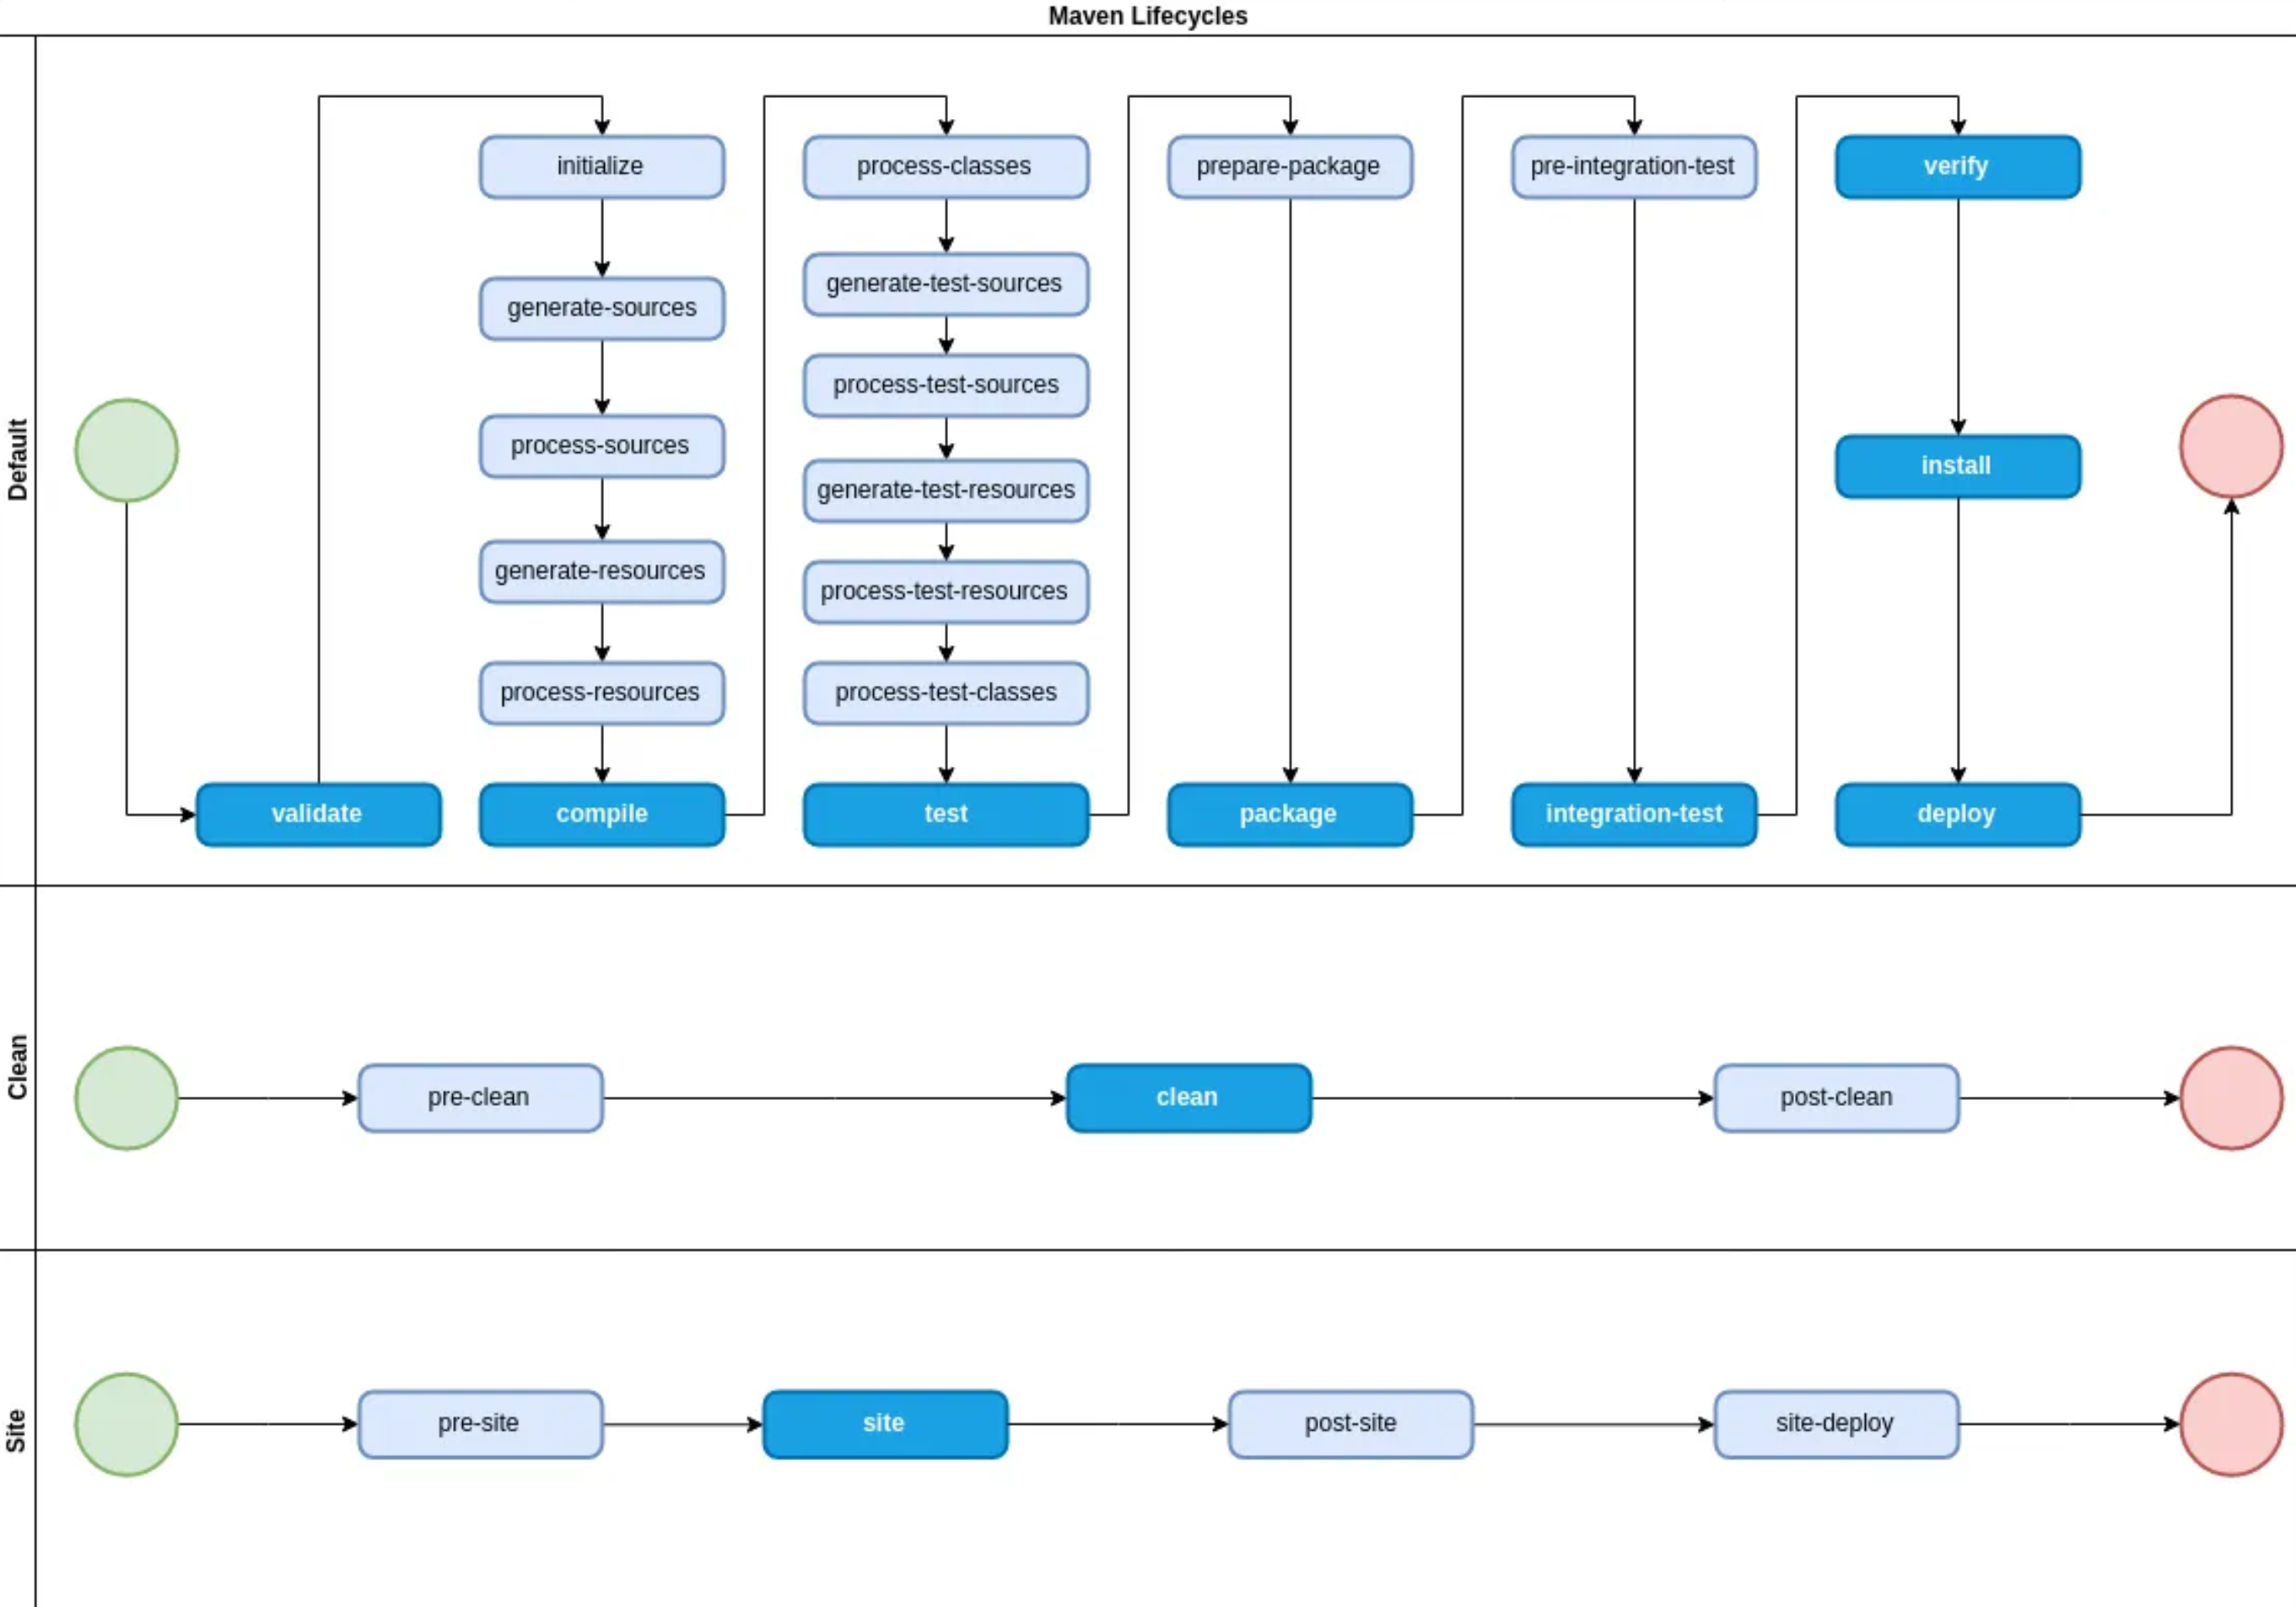
\includegraphics[width=0.8\textwidth]{images/maven-lifecycles.png}
%   \caption{Standard Maven Lifecycles and their goals.} 
%   \footnote{\footnotesize{\url{https://medium.com/@yetanothersoftwareengineer/maven-lifecycle-phases-plugins-and-goals-25d8e33fa22}}}
% \end{figure}

%The key message is, that Maven's view of a software project includes several phases, from generating sources, resources, over compilation to executing tests, caching the result locally and deploying to remote targets.

Maven introduces the notion of life cycles for carrying out tasks on a software project in a certain order.
A life cycle has a name and defines a sequence of phases. 
The phases \texttt{generate-resources} and \texttt{process-resources} are specifically dedicated to generating and packaging resources -- such as data.
The POM follows a single inheritance model such that common configuration options can be placed into a ``parent'' POM.
A typical use case for a parent POM is to configure the repositories to use for dependency resolution and artifact deployment as well as which versions of certain plugins to use.
% \subsection{POM Syntaxes}
Traditionally, POM files are written in XML and tool-chains typically operate on the XML model.
However, nowadays is also possible to write POMs in other popular languages (such as YAML) using the \texttt{polyglot-translate-plugin}\footnote{\url{https://github.com/takari/polyglot-maven}}.

% disabled, focus on the key aspects (by sbin)
% Maven polyglot is the response to the decline in XML's popularity.
% Polyglot is a project that enables the specification of the the project model in many alternative syntaxes, including JSON, YAML or Ruby. \autoref{fig:maven-polyglot} shows how to enable it. During build, each syntax is then converted to the usual pom.xml file.
% Existing pom files can be converted to alternative syntaxes using the following invocation:

% disabled for space reasons
% %\begin{figure}
% \begin{footnotesize}
% \begin{minted}{bash}
% mvn io.takari.polyglot:polyglot-translate-plugin:translate \
%   -Dinput=pom.xml -Doutput=pom.yml
% \end{minted}
% \end{footnotesize}
% %\end{figure}

% \begin{figure}
% \begin{minted}{xml}
% <?xml version="1.0" encoding="UTF-8"?>
% <extensions>
%     <extension>
%         <groupId>io.takari.polyglot</groupId>
%         <artifactId>polyglot-yaml</artifactId>
%         <version>0.7.0</version>
%     </extension>
% </extensions>
% \end{minted}
% \caption{This snippet in \texttt{.mvn/extensions.xml} enables support for \texttt{pom.yml}}
% \label{fig:maven-polyglot}
% \end{figure}

% \subsection{A Model for naming Artifacts}
%In this section we describe Maven's model for naming artifacts.
% Artifacts in Maven are located along a 5 dimensional coordinate system:
Each Maven project is described by a \emph{groupId}, an \emph{artifactId} and a \emph{version} (GAV). 
% Todo check manual newline position
The groupId is typically a reverse domain name such as \texttt{org.myorganiza\newline tion.mydepartment.myproject} and can thus be used to link an artifact to an organization in a Web-compatible way.
By using domains that are under ones own control, unique global identifiers that are nevertheless human-readable are ensured.
Artifact naming can also be leveraged for access control: For example, when publishing artifacts to Maven Central, permission is only granted to upload artifacts whose groupIds start with a specific prefix such as \texttt{org.myorgan\newline ization}.
Maven repositories can be configured to enforce that each version is only published exactly once, thereby ensuring that the exact state of a published dataset is not changed.
%(such as the Maven Central)

To each project GAV, any number of files can be attached. Files are differentiated by the type, such as jar, zip, ttl or nt.bz2, and a classifier, which can be any custom value. For example, in this work we use the classifier \emph{dcat} to tag the RDF metadata datasets to load into the triple store. One way to see a GAV is as a URN for a folder (or archive) which contains files with different names and types.
%\todo{@claus was macht man wenn man mehrere rdf dateien anhängen will?}
% Na halt andere classifier nehmen
Publishing a Maven project usually also attaches the POM file itself. POMs can be designed in a self-contained way such that the creation of artifacts becomes reproducible from the POM itself.

As for repository systems, Maven by default resolves dependencies against the central repository. The plugins we developed as part of this work are published there and can thus be readily reused in Maven builds. In order to not misuse the central repository as a data dump, we set up our own organization-wide repository system instance.
%While datasets can be deployed to the central repository it seems preferably to only do so in conjunction with software that relies on them (such as NLP tools).

% disabled because too long (by sbin)
% The three most fundamental fields are:
% \begin{itemize}
% \item The groupId is typically a domain name such as org.myorganization.mydepartment.myproject and can thus be used to link an artifact to an organization in a Web-compatible way.
% \item The artifactId is used as the name of a relevent unit of work within the group.
% \item The version naturally is an identifier to capture a "snapshot" of that unit of work a certain point in time.
% \end{itemize}
% These fields are often also referred to as the \emph{GAV}. A GAV can be seen as a name for a project, but additional fields are provided to \emph{attach} files to it:
% \begin{itemize}
% \item type: The type of the artifact. Usually a filename extension such as jar, zip or nt.bz2. As a Java-centric convention, if the type is left empty then it defaults to jar. So there is no "empty" type. The pom file itself has type "pom".
% \item classifier: A custom string to discriminate further files published under the same GAV, i.e. a tag. For example, in this work we use the classifier \emph{dcat} to tag the RDF datasets which to load into the triple store.
% \end{itemize}

% \subsubsection{Artifact Syntax}
% Maven coordinates are often represented with the syntax:
% % Some components use a different component order for use cases such as conflict resolution where the version comes last
% \texttt{groupId:artifactId:version[:type[:classifier]]}

% The [] indicate optional fields, so type and classifier may be omitted, but if a classifier is needed, then a type must be given as well.
% Obviously colons (:) must not be used within values for any of the fields.

% %See Maven's Guide to naming conventions for details about how to choose proper values and the valid characters.
% \subsubsection{Maven Coordinates, URNs, Files and Relative URLs}

% disabled due to length (by sbin)
% A maven coordinate can be effectively seen as an URN. We use the prefix \texttt{urn:mvn:} to represent maven coordinates as RDF IRIs.
% Maven coordinates can be unambiguously mapped to HTTP download links.
% The concept of separating naming and resolution of things with URNs is not new. Notably, Life Science Identifiers\footnote{\url{https://www.lsid.info/}} follow a similar pattern.
% %The difference is, that maven artifact resolution is simply HTTP(s)-based:
% Such Maven URNs can thus be converted to relative paths and prefixed with a repository's base URL in order to obtain a download URL.

%
%
% technische details, unwichtig (by sbin)
%  directory names and file names.
% These in turn correspond to relative URLs:
%     The groupId is turned into a directory prefix by replacing all . with /:
%     A filename is derived as follows:
%         If the classifier is absent, then the pattern is artifactId-[version].[type].
%         Otherwise it is, artifactId-[version]-[classifier].[type]
%
% Example without classifier. Lets assume a monthly report is published as a PDF file.
%
%     Coordinate: org.example:report:2024.02.01:pdf:
%     Translates to: org/example/report-2024.02.01.pdf
%
% Example with classifier. Let's assume a monthly report includes multiple files for different aspects such as sales.
%
%     Coordinate: org.example:report:2024.02.01:pptx:sales:
%     Translates to: org/example/report-2024.02.01-sales.pptx
%

%the final candidate URL for resolution.

% disabled because of length (by sbin)
% \subsubsection{Maven Artifact Repository Management Systems}
% Repository managers have emerged as a response to the need for central management of an organization's assets across several programming languages and tools.
% A repository manager provides control over the creation and access over repositories such as for debian, rpm, nodejs, java, ruby packages.
% \autoref{tab:storage} shows how artifact managers store maven artifacts. \emph{Files} means that maven WebDav uploads are directly mapped to physical files and folders on the file system, similar to maven's local repository.
% \emph{Blob} is and \emph{Hash} are storage abstractions. The former is Nexus's binary large object storage, whereas hash means that content is stored in files named according to a hash code of the content, whereas the mapping to paths is kept in a database.

% Artifact naming can be leveraged for access control: For example, when publishing artifacts to maven central\footnote{\url{https://central.sonatype.com/}}, permission is only granted to upload artifacts whose groupIds start with a specific prefix such as \emph{org.example}.
% %GroupId mimicks a domain name

% From a FAIR perspective, file storage has the advantage that it is easy to use. Any web server can publish a folders as static resources, incremental backups can be easily created using tools such as rsnapshot, and repository changes can be tracked with file system watches.



%\section{RDFization of Maven Repository Content}
\section{Adapting Maven for Data Generation and Deployment}
\label{sec:data}
In this section, we present a concrete selection of relevant tasks related to dataset management, representative of similar ones.
% The examples are on the maven4data website
We then provide a brief overview of the Maven plugins used to solve them.

\begin{figure}[!htb]
\centering
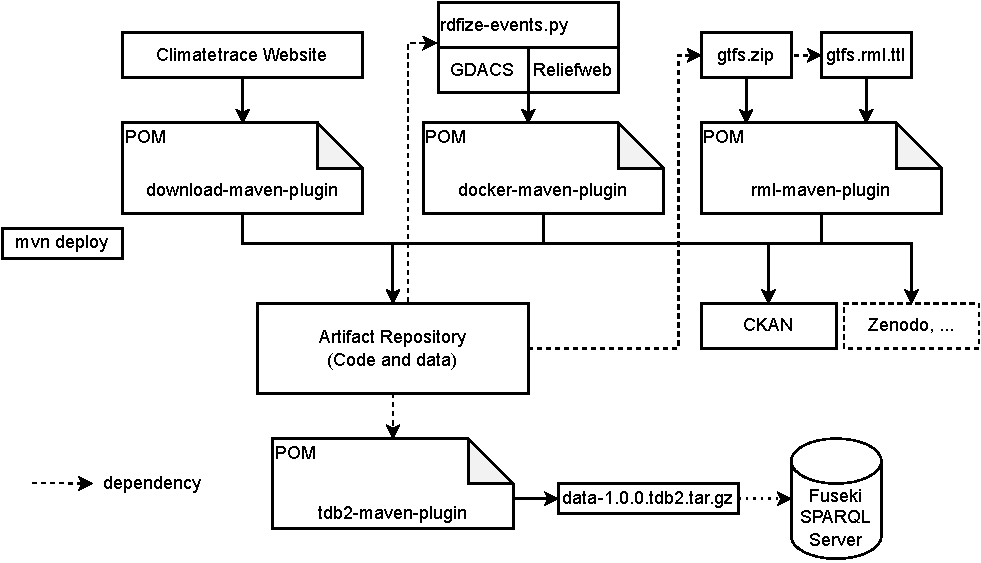
\includegraphics[width=0.8\textwidth]{images/mvn-data-architecture.pdf}
\caption{Architecture with different POM files for unified data processing.}
\label{fig:mvn-arch}
\end{figure}

\autoref{fig:mvn-arch} shows different setups with POM files that make use of different Maven plugins for the creation of artifacts by means of (a) downloading from the Climatetrace\footnote{\url{https://climatetrace.org/data}} website, (b) dockerized execution of a Python script that creates RDF based on data from the GDACS\footnote{\url{https://www.gdacs.org/}} and ReliefWeb\footnote{\url{https://reliefweb.int/}} Web services, and (c) RML mapping execution based on data and mapping files present in the artifact repository. 
Each POM can be executed with \texttt{mvn deploy} which produces the artifacts and uploads them both to a conventional Maven repository as well as to a CKAN instance. Additional plugins could be created for uploading artifacts also to e.g. Zenodo\footnote{\url{https://zenodo.org/}} or Huggingface\footnote{\url{https://huggingface.co/}}.
Furthermore, the \texttt{tdb2-maven-plugin}\footnote{\url{https://github.com/Scaseco/tdb2-maven-plugin}} is capable of creating a TDB2 database file that can be served using a Fuseki SPARQL server.

%\paragraph{Archiving downloads}. The task is to create a maven project whose build result is the downloading a given set of URLs and attaching them as files.
%This effectively enables republishing the content of URLs as maven URNs. This can be realised using the download-maven-plugin\footnote{\url{https://github.com/maven-download-plugin/maven-%download-plugin}}.\todo{Probably artifact download can be removed as its not our work anyway.}

% disabled (by sbin)
% \begin{minted}{yaml}
% build:
%   plugins:
%   - groupId: com.googlecode.maven-download-plugin
%     artifactId: download-maven-plugin
%     configuration: {url: '${input.url}', unpack: false,
%       outputDirectory: '${project.build.directory}',
%       outputFileName: '${output.filename}', skipCache: true}
%     executions:
%     - goals: [wget]
%       phase: process-resources
% \end{minted}

%There are several ways for how this 
%(a) Create one POM per file.
%(b) Attach all files to a single POM.
%(c) Package all downloads into a single archive (e.g. tar) and only attach the tar.

%\paragraph{Attaching files to a maven project}
%\paragraph{Marking files for inclusion in a project distribution}
\subsection*{Marking Files for Inclusion in a Project Distribution}
Files need to be \emph{attached} to a Maven project in order for them to be part of the file set that gets installed locally or deployed remotely.
Many plugins that generate files, such as the Javadoc one, directly support controlling whether to attach the generated files.
The \texttt{build-helper-maven-plugin} is the conventional way for attaching arbitrary files to a maven project using the \texttt{attach-artifact} goal. The GAV is predetermined by the POM, so attached files can only differ in their classifier and type values.
%\todo{(How) to attach generated data? What is supported by your own plugins? @claus (by sbin). The example showed that one just has to list the artifacts under the artifacts key....}

% disabled (by sbin)
% \begin{minted}{yaml}
% build:
%   plugins:
%   - groupId: org.codehaus.mojo
%     artifactId: build-helper-maven-plugin
%     executions:
%     - configuration:
%         artifacts:
%         - {file: '${project.build.directory}/${output.filename}',
%            type: '${output.filetype}'}
%       goals: [attach-artifact]
%       id: attach-artifacts
%       phase: package
% \end{minted}

%\paragraph{Using dockerized data generation}
\subsection*{Docker-based Data Generation}
The \texttt{docker-maven-plugin}\footnote{\url{https://dmp.fabric8.io/}} enables the use of Docker containers from within Maven builds. It supports copying files in and out of containers and requires a running Docker daemon.
For a complete example that runs a Python script to fetch information about disaster events and output them as RDF we refer to our supplemental web page\footnote{\textls[-34]{\url{https://scaseco.github.io/maven4data/how-tos/build-anything-with-docker.html}}}.

%\paragraph{RML Conversion}
\subsection*{RML Conversion}
In~\cite{stadler2023-kgcw-challenge} we presented a system based on our RML Toolkit~\cite{stadler2023-scaling-rml} (rmltk) that rewrites RML mappings to a sequence of extended SPARQL queries.
Likewise, we wrapped this system as a Maven plugin.
To use the system, two dependencies have been specified in the POM: one to an artifact containing the CSV source data, and one containing the RML mapping rules.
Then, the \texttt{rml-maven-plugin} is specified in the plugin section, together with an rmltk-specific configuration (also detailed inside the POM).
When Maven is called with process-resources, the dependencies and the plugins will be downloaded (unless they are already cached) and the mapping will execute.
A complete example is available on GitHub\footnote{\url{https://github.com/Scaseco/resource-gtfs-bench-rml/}}.

% disabled (by sbin)
% \begin{minted}{yaml}
% dependencies:
% - {groupId: org.aksw.data.gtfsbench, artifactId: gtfsbench-csv-1, version: 0.0.1-SNAPSHOT,
%   type: zip}
% - {groupId: org.aksw.data.gtfsbench, artifactId: mapping, version: 0.0.1-SNAPSHOT,
%   type: rml.ttl}
% build:
%   plugins:
%   # Omitted for brevity: Copying of dependencies to ${data.workdir}
%   - groupId: org.aksw.maven.plugins
%     artifactId: rml-maven-plugin
%     version: 0.9.0
%     executions:
%     - configuration:
%         outputFile: ${output.path}
%         outputFormat: ${output.filetype}
%         workDirectory: ${data.workdir}
%         mappings:
%         - {type: file, value: '${data.workdir}/mapping.rml.ttl'}
%       goals: [rml]
%       phase: process-resources
% \end{minted}

%\paragraph{RDF generation with SPARQL Queries}
\subsection*{RDF generation with SPARQL Queries}
We also created the \texttt{sparql-maven-plugin} to enable running SPARQL statements against an embedded triple store.
This enables loading of datasets as well as producing RDF with SPARQL CONSTRUCT queries as part of the build process.
The configuration is similar to that of the \texttt{rml-maven-plugin}
%\todo{@claus rpt plugin? or rml plugin?}
except that SPARQL queries can be provided as string and files.
This plugin can be used to produce VoID, DCAT and PROV metadata.
A crucial aspect is that Maven coordinate URNs of the POM can be used as the dataset identifier.

%\paragraph{Deploying to CKAN}
\subsection*{Deploying to CKAN}
CKAN\footnote{\url{https://ckan.org/}} is a popular open-source open data portal software for the storage and distribution of data. It has an API for uploading data and metadata.
We created the \texttt{ckan-maven-plugin} which enables uploading files to CKAN.
Several fields for the POM are directly mapped to fields in CKAN, such as: name, description and license. The plugin can be used in addition to any other plugins that carry out deployments.
Typically, all deployments are executed in the \texttt{deploy} phase. In general, a Maven build can be designed such that properties and profiles are provided to control which (sub)sets of plugins to execute. These mechanisms can be leveraged to carry out only specific deployments.
%
% disabled (by sbin)
% \begin{minted}{yaml}
% build:
%   plugins:
%     - groupId: org.aksw.maven.plugins
%       artifactId: ckan-maven-plugin
%       version: ${ckan-maven-plugin.version}
%       executions:
%         - id: ckan-upload
%           phase: deploy
%           goals: [upload]
%           configuration:
%             ckanUrl: https://your.ckan.instance/
%             serverId: your.ckan.serverId
%             datasetId: My Dataset Label
%             resourceId: ${project.artifactId}
%             fileName: ${output.path}
%             organizationId: my-ckan-org
%             author: Your Name
% \end{minted}
%
%Credentials for CKAN access are stored in the \texttt{\$HOME/.m2/settings.xml} file, as is customary for all credentials used by maven connectors.
The plugin supports reading (possibly encrypted) CKAN API keys from Maven's \texttt{settings.xml} file, which is Maven's default place for user-level passwords.
Note, that whether and how conventional dependencies can be (reasonably) resolved against a CKAN instance is future work.
%Note, that there is no established mapping procedure from Maven coordinates to CKAN entries, and 
More details about the configuration of the CKAN plugin is available on GitHub\footnote{\url{https://github.com/Scaseco/ckan-maven-plugin}}.
%\begin{minted}
%<server>
%  <id>your.ckan.serverId</id>
%  <username>your_username</username>
%  <password>your-optionally-encrypted-ckan-api-key</password>
%</server>
%\end{minted}


%\paragraph{Loading a triple store from dependencies}
\subsection*{Loading a Triple Store from Dependencies}
% disabled (by sbin)
% \begin{figure}
% \begin{footnotesize}
% \begin{minted}{yaml}
% modelVersion: 4.0.0
% parent: {artifactId: aksw-data-deployment, groupId: org.aksw.data.config,
%          version: 0.0.8, relativePath: ''}
% groupId: org.aksw.maven4data.examples
% artifactId: my-example-kg
% version: 1.0.0
% packaging: pom
% properties:
%   baseDir: ${project.build.directory} # Declaration for CWL interoperability!

% dependencies:
% - { groupId: org.coypu.data.disasters, artifactId: disasters,
%     version: 0.20240312.1842, type: nt.bz2 }
% - { groupId: org.aksw.moin, artifactId: moin,
%     version: 1.20220502.0, type: ttl.bz2 }
% build:
%   plugins:
%   - { groupId: org.aksw.maven.plugins, artifactId: tdb2-maven-plugin,
%       version: 0.0.1-SNAPSHOT }
%     executions:
%     - goals: [load]
% \end{minted}
% \end{footnotesize}
% \caption{pom.yml file for the creation of a TDB2 database archive.}
% \label{fig:tdb2-yml}
% \end{figure}
% %\end{minipage}

%\autoref{tdb2-yml} demonstrates the generation of a \emph{tdb2.tar.gz} for the provided RDF dependencies.\todo{get rid of snapshot}
We have created the \texttt{tdb2-maven-plugin}, that uses Apache Jena to convert RDF data into a TDB2 database suitable for use with Apache Jena.
%can be placed into a profile in order to not create the database archive by default. This way, \texttt{mvn deploy} will only deploy the \texttt{pom.xml} file without the data. This saves space in the archive and yet allows re-creation of the database any time in the future, such as when the need arises to perform evaluation on historic data.
To use it, the RDF datasets are specified as dependencies in the Maven POM, and the tdb2-maven-plugin is referenced in the build plugins section.
A limitation is, that Maven does not natively support the automatic build of missing artifacts based on a reference to a POM that could build those.
It may be possible to create further plugins that carry out such tasks by analyzing the dependency tree but but this is open to future work.

%of the database when using such a Maven project as a dependency in another project.
%client-side recreation of artifacts when referencing such a pom as a dependency.


\section{Synchronization of Metadata}
\label{sec:mvn-sync}
\begin{figure}[!htb]
\centering
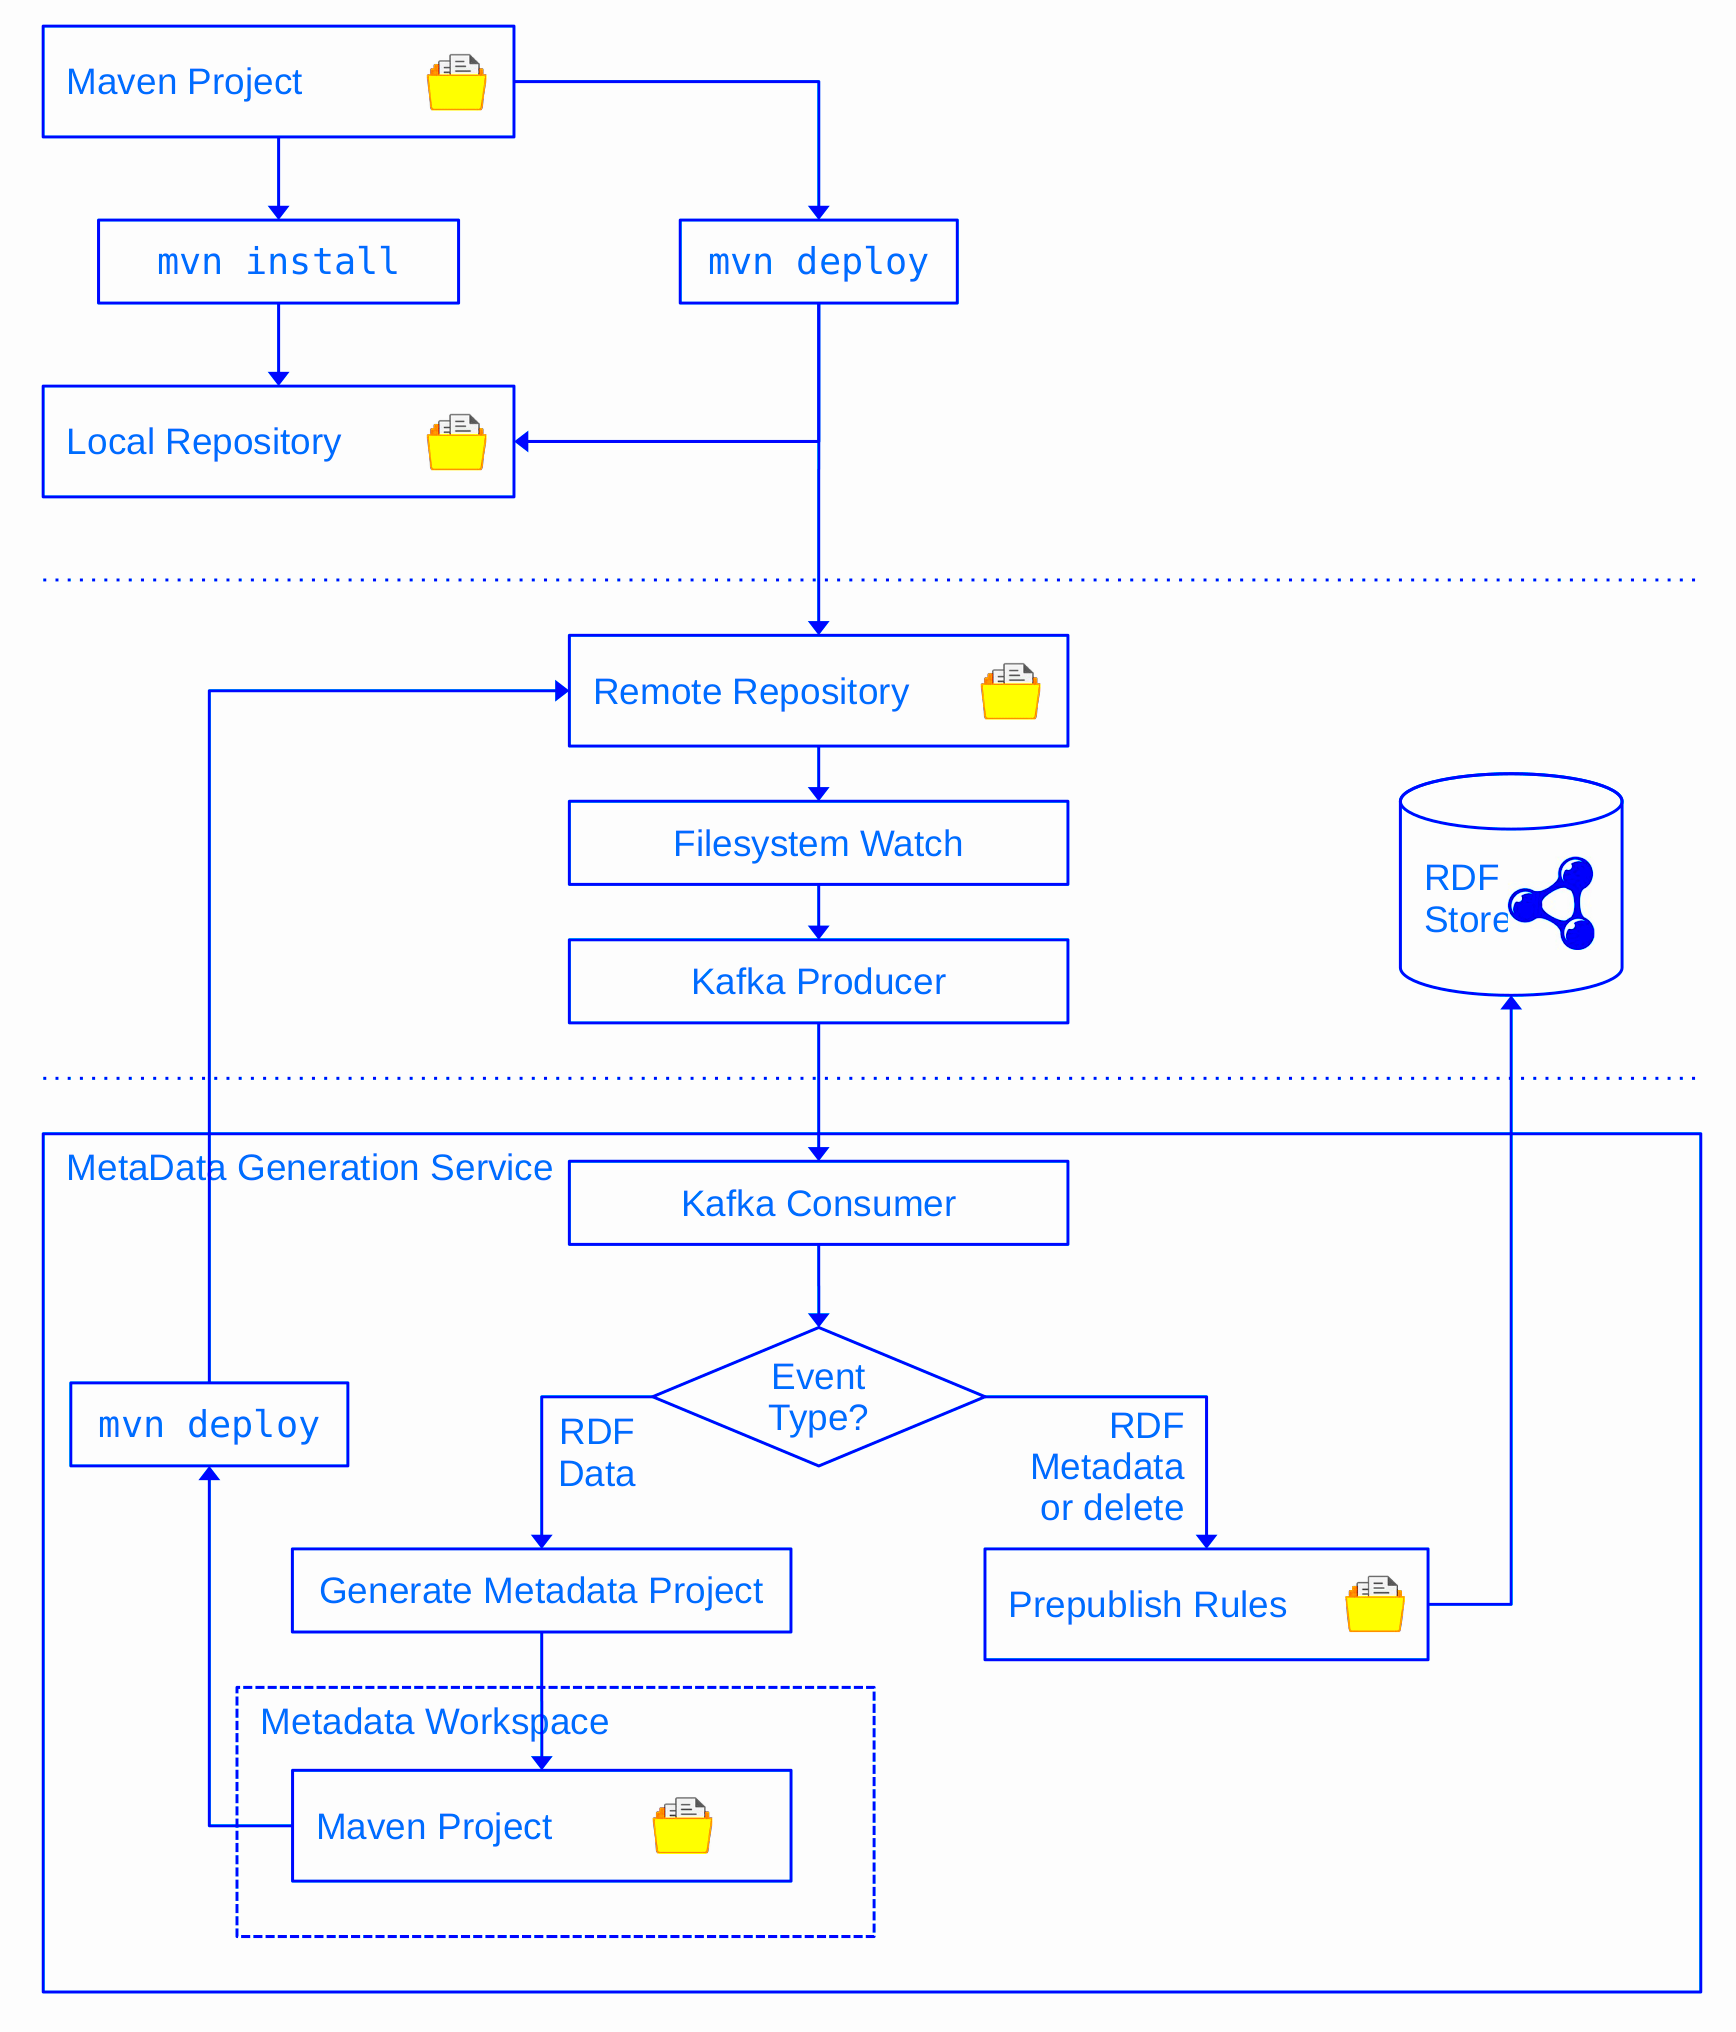
\includegraphics[width=0.7\textwidth]{images/2024-03-01-mvn-sync-architecture.png}
\caption{Architecture of our Maven-RDF-Sync approach.}
\label{fig:mvn-rdf-sync-arch}
\end{figure}
In the previous sections, we looked at how to build a Maven project that can deploy data.
In this section, we present \emph{mvn-rdf-sync}, an approach that after deployment of RDF data automatically generates and deploys metadata.
%VoID, PROVO and DCAT
The process is depicted in~\autoref{fig:mvn-rdf-sync-arch}.
%\todo{Add numbers to the picture}
The steps are:
\begin{enumerate}
\item A trigger on a Maven repository's file system detects changes and publishes appropriate events.
\item An event consumer examines the event type. If it is an RDF data artifact, then one or more Maven projects for metadata generation are created. This step essentially creates an instance from a Maven template project\footnote{\textls[-27]{\url{https://github.com/Scaseco/mvn-rdf-sync/blob/main/v3/dcat-generator/pom.xml}}}, using parameters from the changed artifact's POM.
By convention, we use the classifier \texttt{dcat} to indicate artifacts with DCAT metadata.
In principle, a future version of the setup could support attached RO-Crate files.
\item The metadata project is then deployed as usual using \texttt{mvn deploy}.
\item The change to the file system is detected and another event is sent.
\item This time the event consumer sees the RDF file with the \texttt{dcat} classifier and can choose the flow for publishing metadata.
In order to prevent arbitrary metadata to end up being published, metadata artifacts can be filtered by trusted groupIds.
\item A sequence of pre-publish rules, essentially SPARQL update queries, is used to transform the raw metadata into the final one. These rules are used to convert Maven URNs to resolvable download URLs and to run queries that for fixing any issues with previously published metadata.
\item Finally, the data ends up in the triple store for access. The metadata is loaded into a graph that matches the metadata artifact.
\item The data is now (publicly) accessible via SPARQL. Tools, such as Yasgui\footnote{\url{https://yasgui.triply.cc/}}, can be used to query and visualize the content.
\end{enumerate}

\begin{figure}[!htb]
\centering
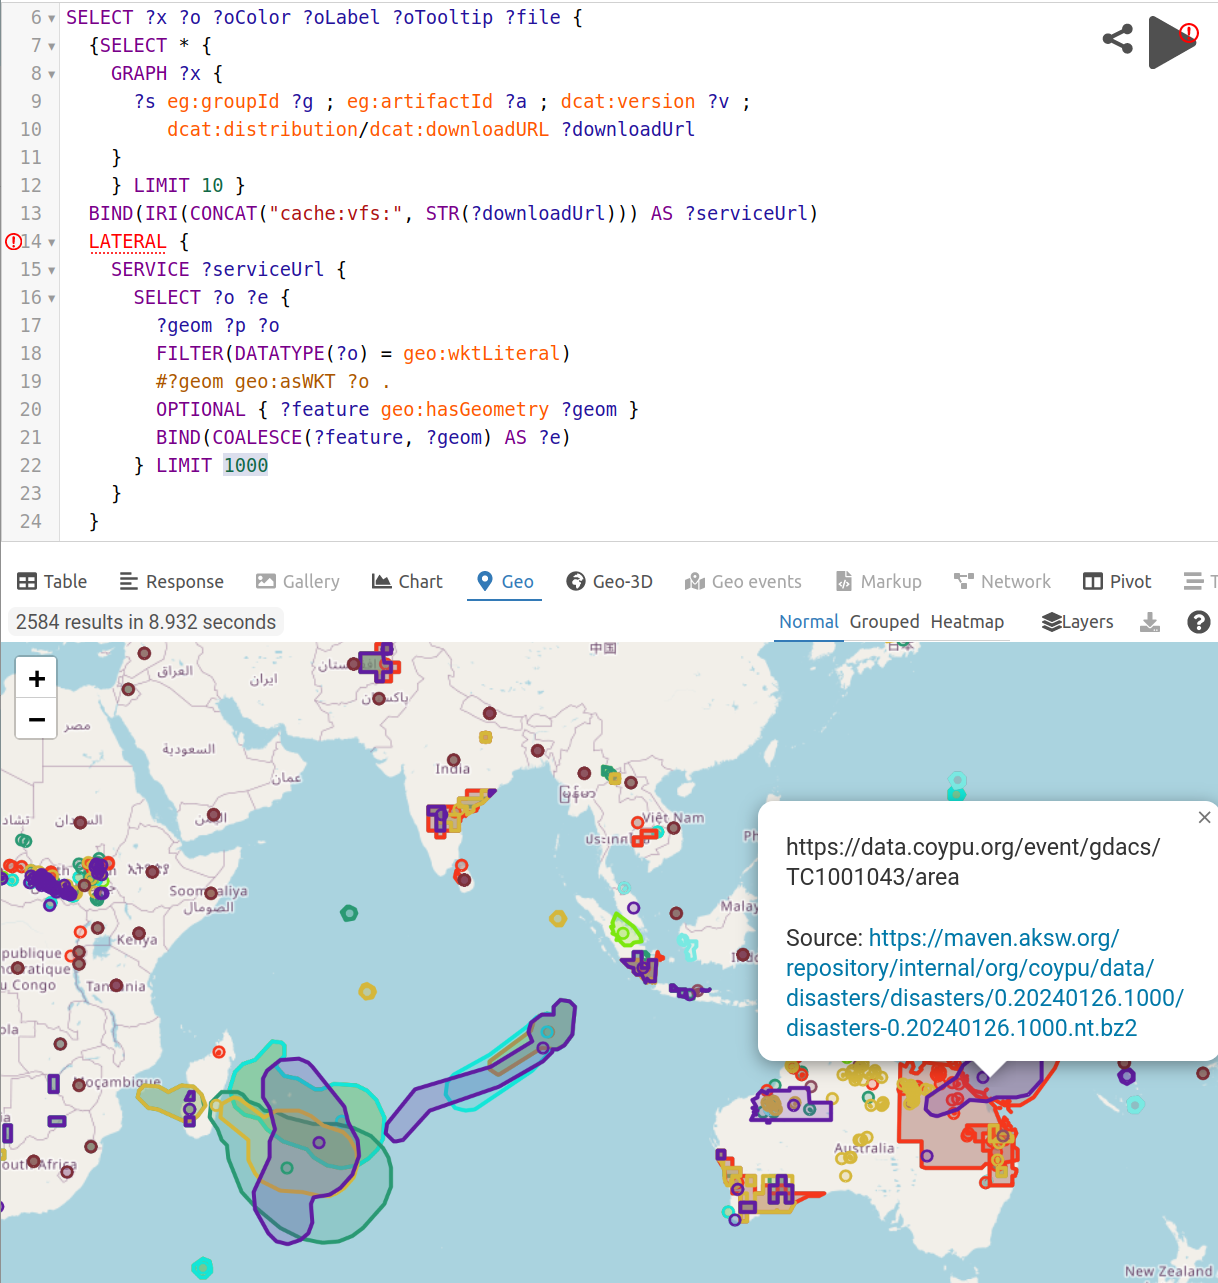
\includegraphics[width=0.8\textwidth]{images/Screenshot from 2024-03-18 01-11-50.png}
\caption{Visualization of data catalog content on a map via SPARQL.}
\label{fig:cat-content}
\end{figure}
%2024-03-03-yasgui-maven.png

A screenshot of our online demo\footnote{\url{https://scaseco.github.io/maven4data/online-demo.html}} is shown in~\autoref{fig:cat-content}.
It shows how the DCAT metadata in the triple store synchronized with the Maven repository can be queried with SPARQL and plotted on a map with Yasgui. As the mvn-rdf-sync process also generates VoID metadata, it is also possible to e.g. filter datasets by the used classes and properties. The datasets are identified by \texttt{urn:mvn:} URNs, such that a transfer of the repository to a different URL does not invalidate any dataset identifiers.

It is a design decision whether to use a single Maven template project to capture multiple metadata aspects, such as VoID, DCAT and PROV-O, or whether to maintain individual Maven templates for each of them. For the prototype we went with the former approach, but as the system grows it is likely that we will switch to the latter due to better modularity.
The metadata project includes generation of the provenance triples that state that the original artifact was generated by an activity whose plan is the URN of the original artifact's POM.
If that POM was designed to be self-contained then downloading the POM and running \texttt{mvn package} will re-run the build. If the POM was designed for reproducible builds then the output artifacts will match the deployed ones. For non-reproducible builds, such as those that consume live data from APIs, one should typically adjust the groupId and version appropriately before creating custom builds.

\section{Resources and Evaluation}
\label{sec:eval}
We have set up the \emph{Maven4Data} website with guides and examples that we have shown in this paper, demonstrating the effectiveness of the approach.

A relevant question is to what extent our mvn-rdf-sync approach degrades the performance of a filesystem-based repository due to overhead of file system watches. For this purpose we devised the ``repo-bench''\footnote{\url{https://github.com/Scaseco/mvn-rdf-sync/tree/main/benchmark}} benchmark:
We use a python script to generate a Maven project with $n=500$ sub modules, where each sub module has a corresponding RDF dataset. The triple count for the $i-th$ project is $i \times 1000$ triples, with $1 \leq i \leq n$, amounting to ${\frac{n}{2}} \times (n + 1) \times 1000 = 125.250.000$ triples in total with a size of 14.2G of data.

We measure the time it takes to install the poms with and without the file system watch active.
The experiment was carried out on a Dell XPS 9720 notebook with the following specs: CPU: Intel i9-12900HK CPU, SSD: NVMe PC801 NVMe SK hynix 2TB, RAM: 64GB.
We use the following basic watch to check for changes to the file system:

{\scriptsize
% too much detail/technical? (comment by sbin)
\begin{minted}{bash}
inotifywait "$HOME/.m2/repository" --recursive --monitor --format '%e %w%f' \
  --event CLOSE_WRITE --event DELETE | xargs -n 1 -P 0 bash -c 'echo  "$@"; sleep 1' _ {}
\end{minted}
}
The flag \texttt{-P 0} indicates to spawn a fresh process for each line emitted by inotifywait, such that maximum parallelism is utilized.
The finding is that regardless whether the following watch is active or not, running \texttt{mvn install} takes $\approx$20 seconds, which indicates that the watch itself does not impact the performance significantly. However, more extensive analysis is needed for how real-world workloads affect overall system performance.


%\todo{Evaluate and compare inotifywait with and without filter regex}


%\begin{minipage}{\linewidth}
%[language=yaml, caption=POM file for the creation of a TDB2 database.]

\section{Conclusions and Future Work}
\label{sec:conclusions}
This work is motivated by the multitude of solutions in the field of data management and the pursuit of a ``minimal'' one that is open source, can run locally, is extensible, and interoperable with Semantic Web technology.
% mature, file system based
In pursuit of such a solution, we took a deep dive in the Apache Maven ecosystem.
%we recapped the life cycle of data artifacts under an ETL process and showed that it can be mapped to the life cycle of Apache 
We presented a selection of use cases where the life cycle of data artifacts can be mapped to a Maven build process. A set of Maven plugins was devised for streamlining the generation of RDF and for the deployment of artifacts to CKAN instances.
We showed that Maven's build specifications can be designed in a way that makes them self-contained w.r.t. versioning, data processing and deployment.
The fact that upon deployment the POM is archived as well makes the process self-documenting and can be leveraged for reproducibility.
Based on our findings, we devised the \emph{mvn-rdf-sync} system, which listens to changes to Maven repository and triggers RDF metadata generation (via generated Maven projects) when RDF datasets are uploaded.
We assembled at the Website \emph{Maven4Data}
%\footnote{\url{https://scaseco.github.io/maven4data/}}
where we provide additional information and examples.
We also compared Maven to CWL and found that these systems are complementary: Maven's scope is more narrow than that of general workflow engines, yet it provides several features that are highly useful for versioning, packaging and deploying artifacts.

% both deployment of the output artifacts to different locations (WebDAV, CKAN) as well
%makes the data processing process self-contained.

Future work is along the following lines:
(1) Investigation of creating Research Object Crates from Maven.
%For example, would it make sense to build creates with Maven,interoperable with existing artifact repository systems.
(2) Analysing the feasibility of Maven plugins that can deploy to further popular public archives.
For (2), it needs to be investigated to what extent Maven's coordinate system can be bridged with the artifact naming system provided by those archives. For example, Zenodo provides APIs for custom tags which could be exploited for that purpose.
%and searching over them which could be exploited.

%\section*{Acknowledgments}
%The authors acknowledge the financial support by the German Federal Ministry for Economic Affairs and Climate Action in the project Coypu (project number 01MK21007A) and by the German Federal Ministry for Digital and Transport in the Project Moby Dex (project number 19F2266A).

%\pagebreak

%\bibliographystyle{splncs04}
%\bibliography{bibliography}




\section{Conclusions and Future Work}



\end{document}
